\documentclass[12pt, a4paper]{article}
\usepackage[utf8]{inputenc}
\usepackage{amsmath}
\usepackage{relsize}
\usepackage{array}
\usepackage{xcolor}
\usepackage{courier}
\usepackage{listings}
\lstset{basicstyle=\footnotesize\ttfamily,breaklines=true}
\lstset{framextopmargin=50pt,frame=bottomline}
\usepackage{tikz}
\usetikzlibrary{calc}
\usepackage{graphicx}
\graphicspath{ {./images/} }
\usepackage{multirow}

\title{CEG3155A Assignment 4}
\author{Jake Wang/*}
\date{\today}

\begin{document}
	\maketitle
	
	\section*{Question I}
	\subsection*{Part a}
	\begin{align*}
		f_1(x_1, x_2, x_3) &= \sum{m(1, 2, 4, 7)} \\
		&= \prod{M(0, 3, 5, 6)} \\
		&= (x_1 + x_2 + x_3)(x_1 + x_2' + x_3')(x_1' + x_2 + x_3')(x_1' + x_2' + x_3)
	\end{align*}
	
	Since we are using a NOR-NOR PLA, we need to convert the equation to
	NOR-only form:
	\begin{align*}
		f_1(x_1, x_2, x_3) &= (x_1 + x_2 + x_3)(x_1 + x_2' + x_3')(x_1' + x_2 + x_3')(x_1' + x_2' + x_3) \\
		&= ((x_1 + x_2 + x_3)' + (x_1 + x_2' + x_3')' + (x_1' + x_2 + x_3')' + (x_1' + x_2' + x_3)')'
	\end{align*}
	
	PLA Circuit Diagram:
	\begin{center}
		\begin{tikzpicture}
			\node(graphic)
			{
				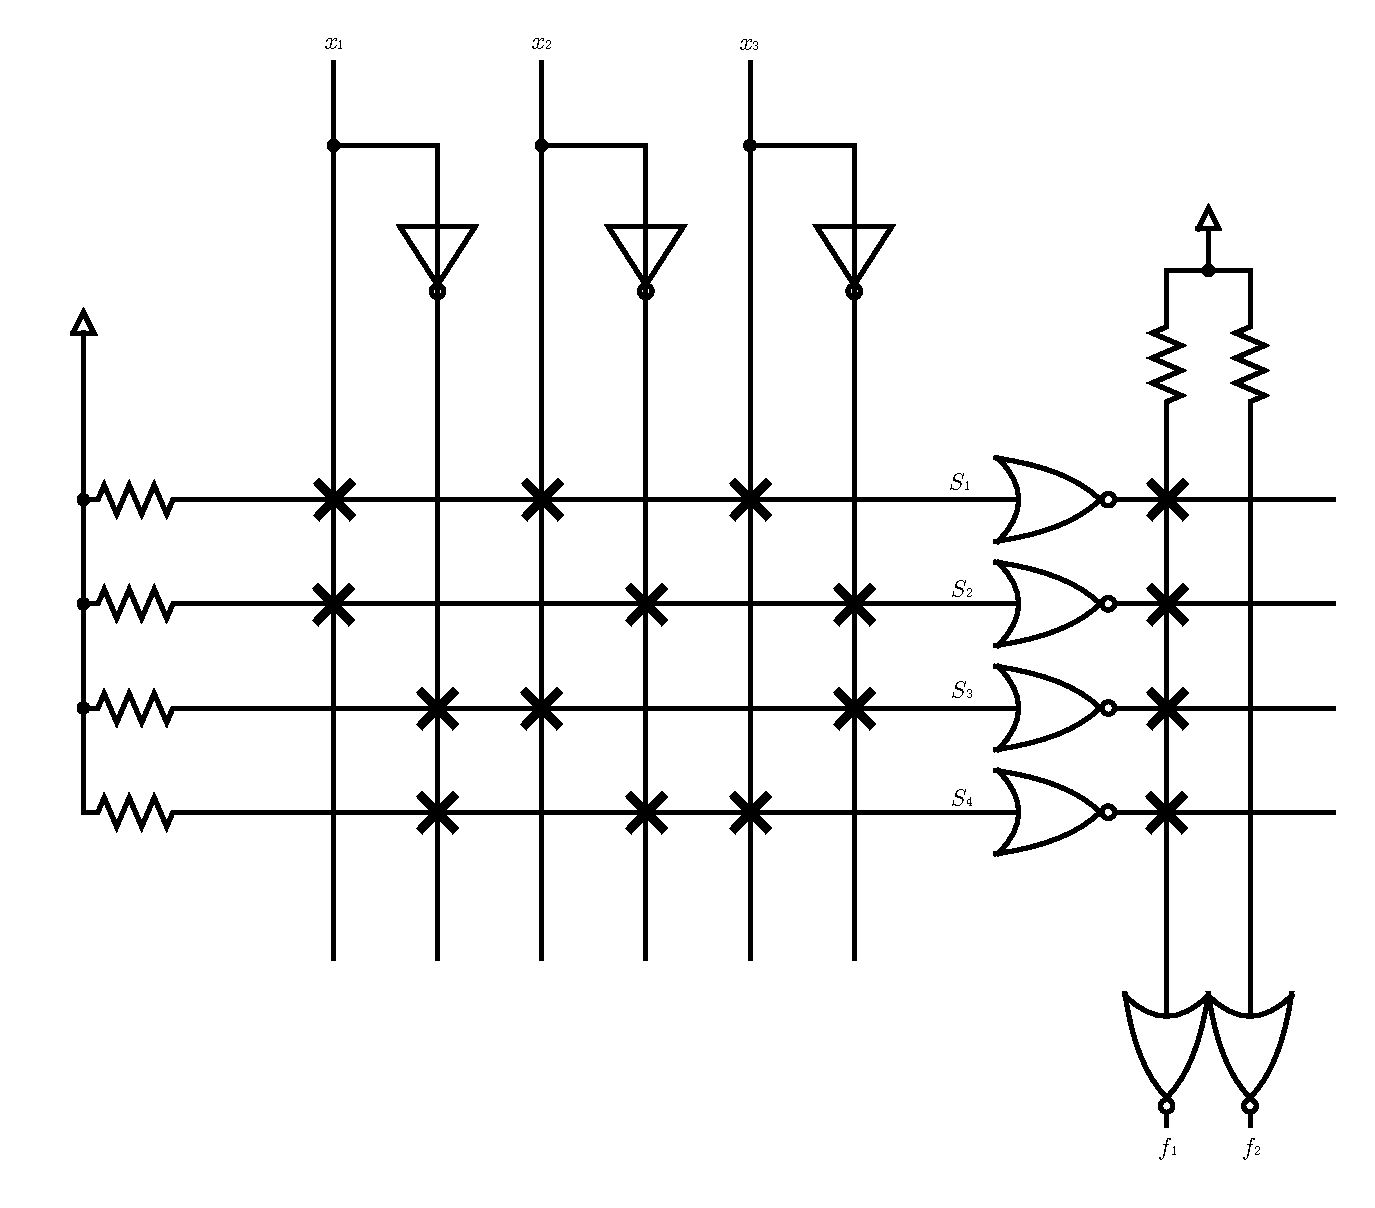
\includegraphics[scale=0.65]{Q1a.pdf}
			};
		\end{tikzpicture}
	\end{center}
	
	\subsection*{Part b}
	PLA Circuit Diagram:
	\begin{center}
		\begin{tikzpicture}
			\node(graphic)
			{
				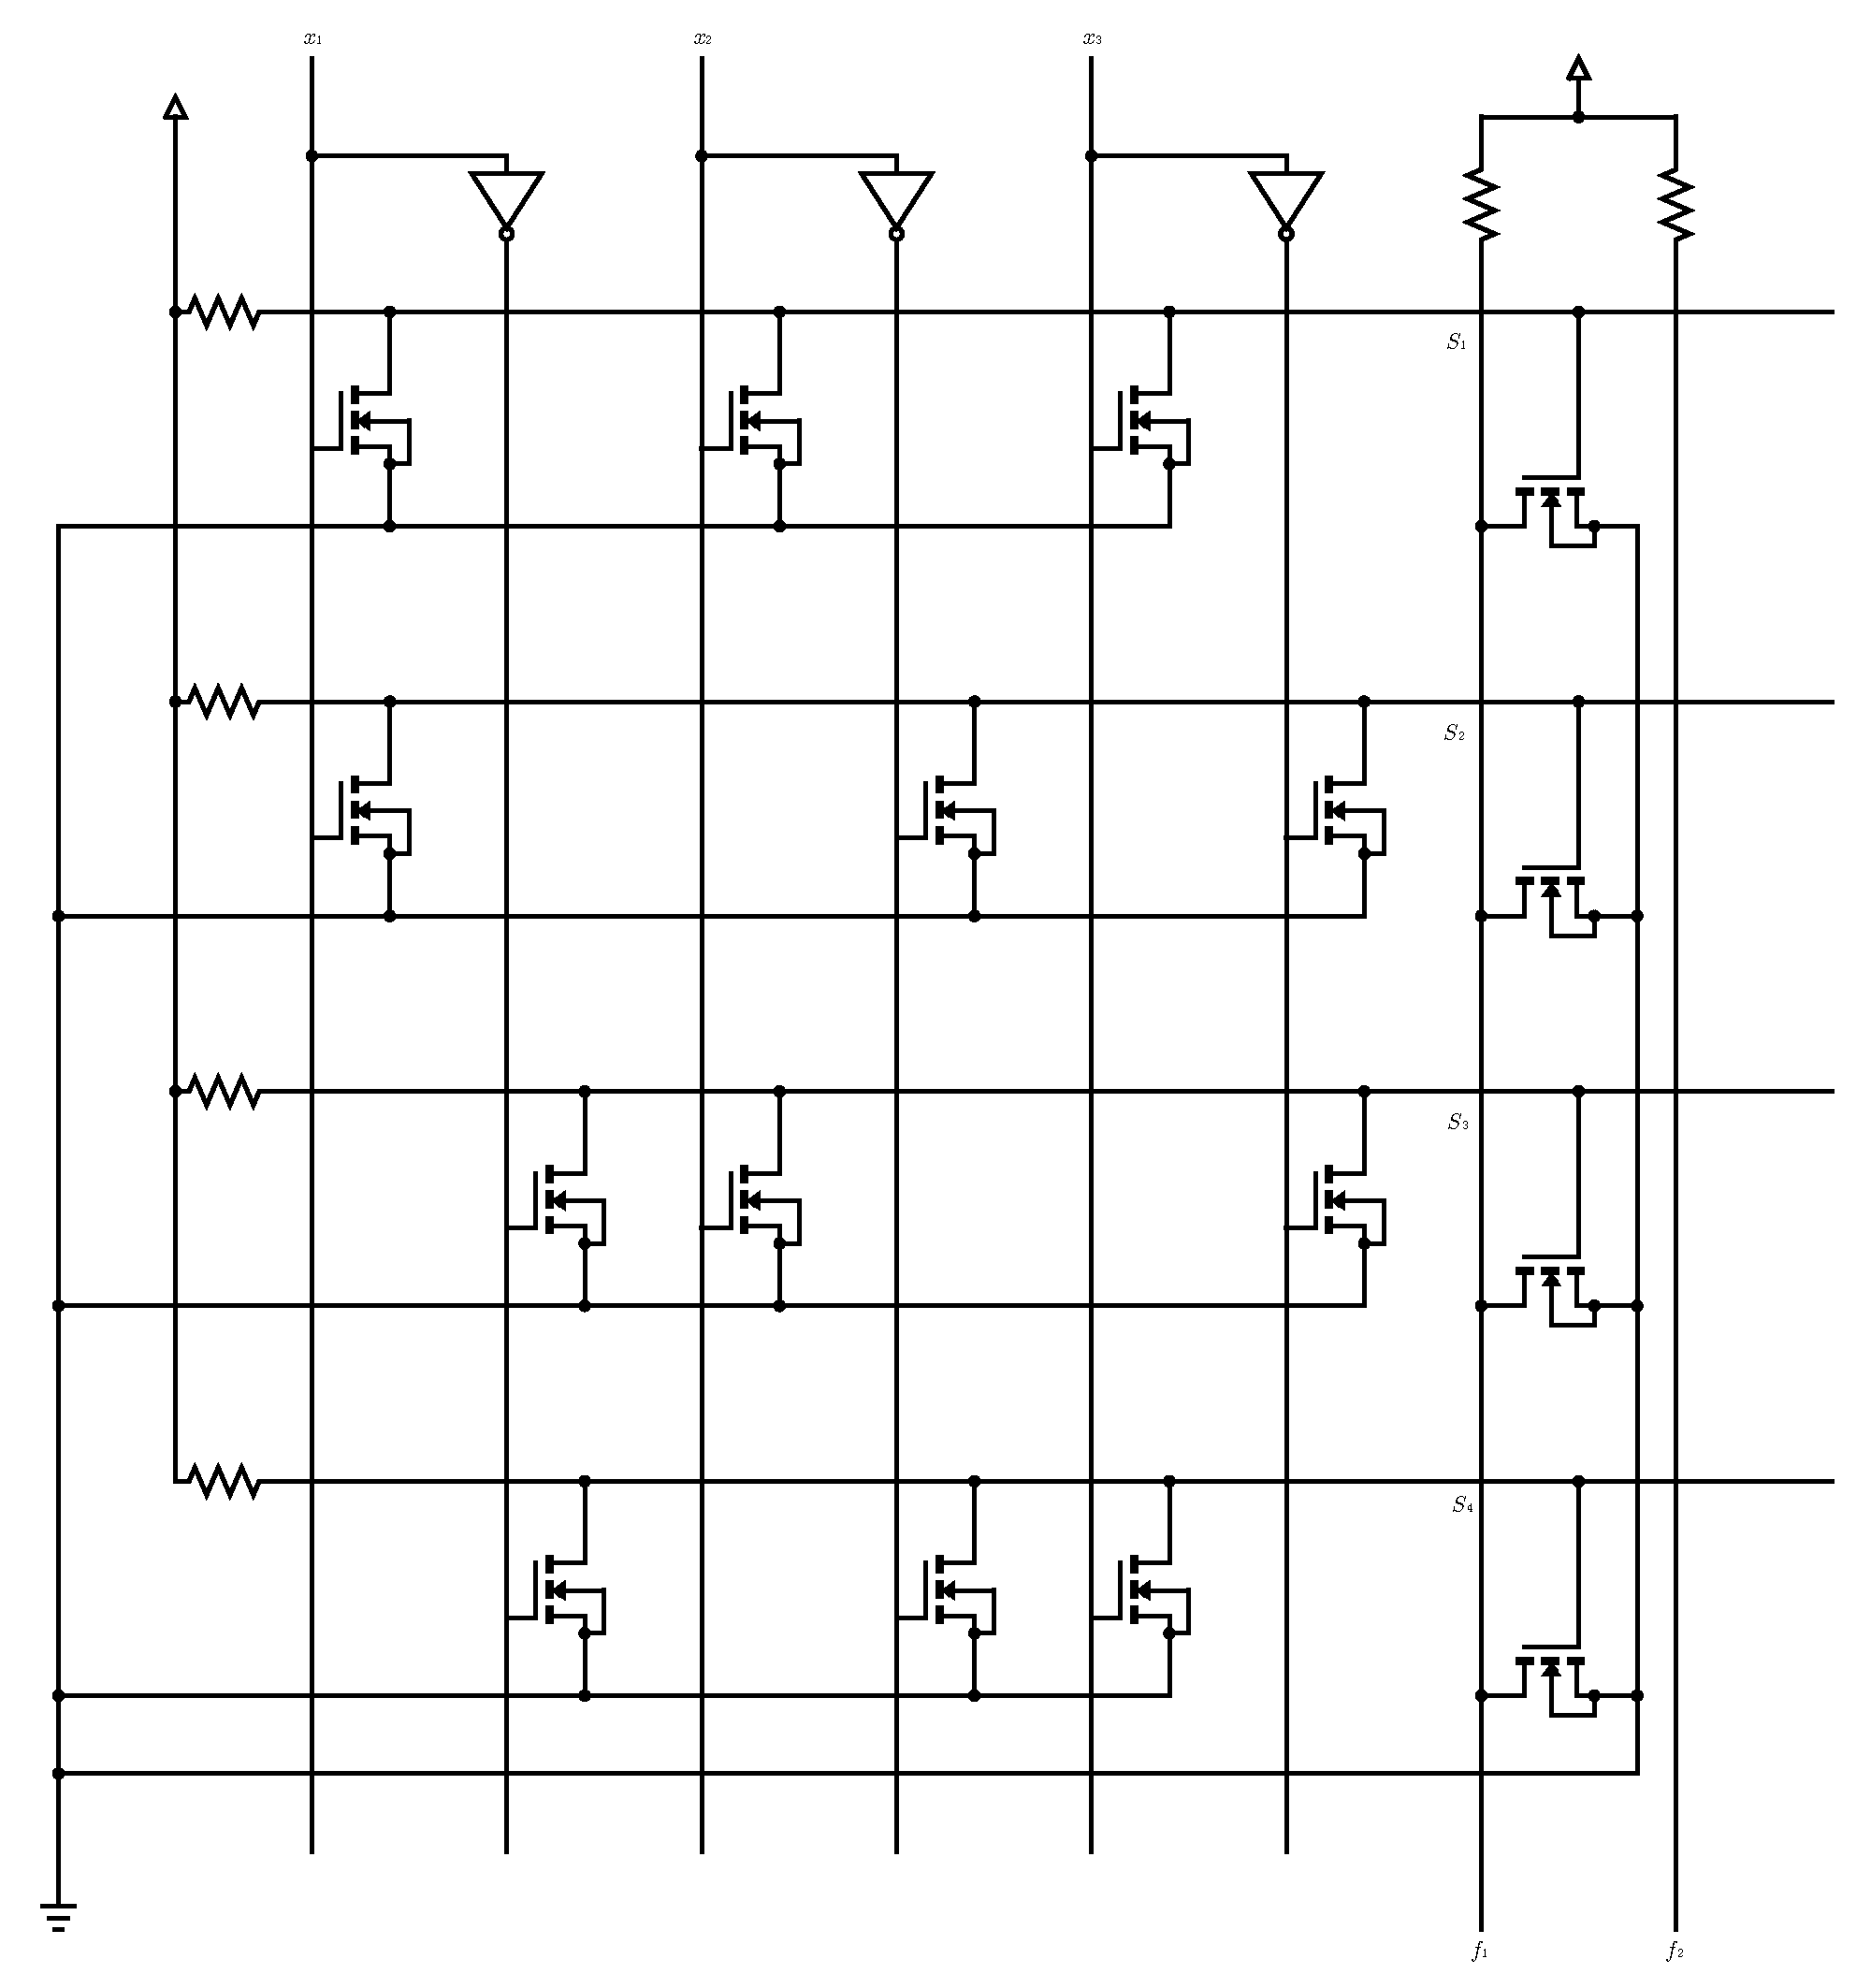
\includegraphics[scale=0.42]{Q1b.pdf}
			};
		\end{tikzpicture}
	\end{center}
	
	\subsection*{Part c}
	Use Shannon Expansion on $f$ with respect to $x_2$:
	\begin{align*}
		f &= x_1x_2x_4 + x_2x_3x_4' + x_1'x_2'x_3' \\
		&= x_2(x_1x_3 + x_3x_4') + x_2'(x_1'x_3')
	\end{align*}
	
	Denote $f_1 = x_1x_3 + x_3x_4'$ and $f_2 = x_1'x_3'$. \\
	
	Then $x_2$ can be treated as a 2-to-1 MUX, which can be implemented
	with the third LUT, whereas $f_1$ and $f_2$ can be implemented with
	other two LUTs.
	
	\begin{center}
		\begin{tikzpicture}
			\node(graphic)
			{
				\includegraphics[scale=0.7]{Q1c.pdf}
			};
		\end{tikzpicture}
	\end{center}
	
	\section*{Question II}
	\subsection*{Part a}
	Relabel the flow table:
	\begin{center}
		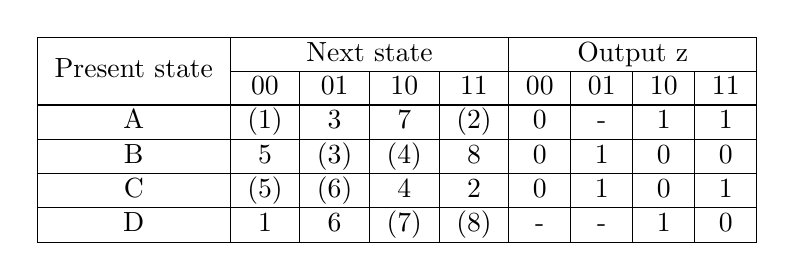
\begin{tikzpicture}
			\node(table)
			{
				\begin{tabular}{| c | c | c | c | c | c | c | c | c | c |}
					\hline
					\multirow{2}{*}{Present state} & \multicolumn{4}{c |}{Next state} & \multicolumn{4}{c |}{Output z} \\
					\cline{2-9} & $00$ & $01$ & $10$ & $11$ & $00$ & $01$ & $10$ & $11$ \\
					\hline
					A & (1) & 3 & 7 & (2) & 0 & - & 1 & 1 \\
					\hline
					B & 5 & (3) & (4) & 8 & 0 & 1 & 0 & 0 \\
					\hline
					C & (5) & (6) & 4 & 2 & 0 & 1 & 0 & 1 \\
					\hline
					D & 1 & 6 & (7) & (8) & - & - & 1 & 0 \\
					\hline
				\end{tabular}
			};
		\end{tikzpicture}
	\end{center}
	
	Draw the transition diagram for current states:
	\begin{center}
		\begin{tikzpicture}
			\node(graphic)
			{
				\includegraphics{Q2aTD.pdf}
			};
		\end{tikzpicture}
	\end{center}
	
	The diagnol transition cannot be eliminated without adding new states.
	Expand encoding to 3-bit space.
	
	Three states E, F and G are added.
	\begin{center}
		\begin{tikzpicture}
			\node(graphic)
			{
				\includegraphics{Q2aTDnew.pdf}
			};
		\end{tikzpicture}
	\end{center}
	$$CD \rightarrow CE, ED$$
	$$BD \rightarrow BF, FD$$
	$$BC \rightarrow BG, GC$$
	
	New flow table:
	\begin{center}
		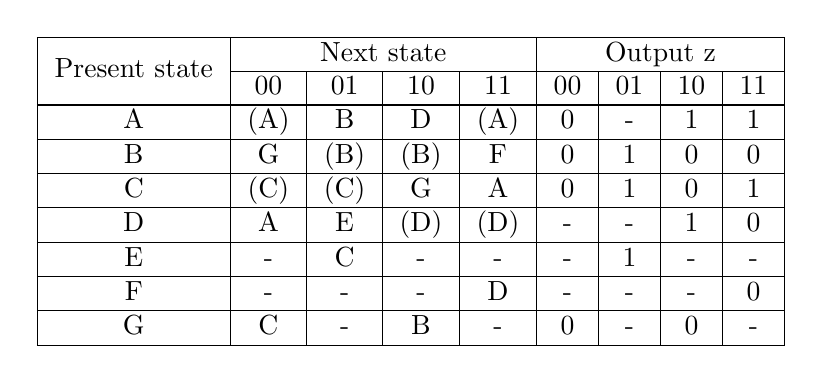
\begin{tikzpicture}
			\node(table)
			{
				\begin{tabular}{| c | c | c | c | c | c | c | c | c | c |}
					\hline
					\multirow{2}{*}{Present state} & \multicolumn{4}{c |}{Next state} & \multicolumn{4}{c |}{Output z} \\
					\cline{2-9} & $00$ & $01$ & $10$ & $11$ & $00$ & $01$ & $10$ & $11$ \\
					\hline
					A & (A) & B & D & (A) & 0 & - & 1 & 1 \\
					\hline
					B & G & (B) & (B) & F & 0 & 1 & 0 & 0 \\
					\hline
					C & (C) & (C) & G & A & 0 & 1 & 0 & 1 \\
					\hline
					D & A & E & (D) & (D) & - & - & 1 & 0 \\
					\hline
					E & - & C & - & - & - & 1 & - & - \\
					\hline
					F & - & - & - & D & - & - & - & 0 \\
					\hline
					G & C & - & B & - & 0 & - & 0 & - \\
					\hline
				\end{tabular}
			};
		\end{tikzpicture}
	\end{center}
	
	State assignment:
	$$A=000$$
	$$B=001$$
	$$C=100$$
	$$D=010$$
	$$E=110$$
	$$F=011$$
	$$G=101$$
	
	Excitation table:
	\begin{center}
		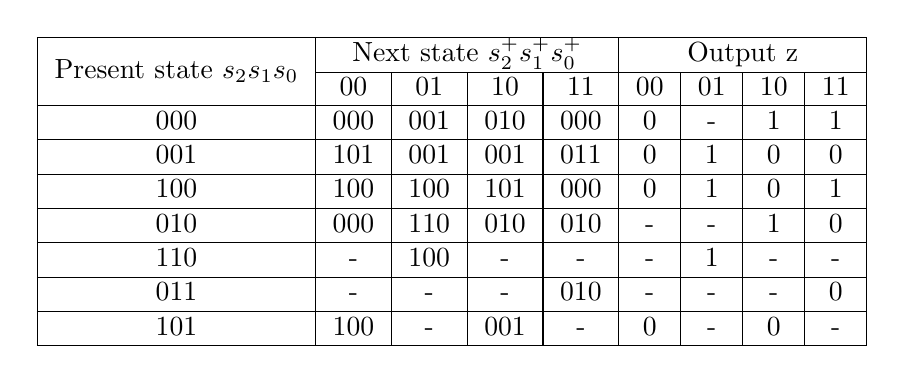
\begin{tikzpicture}
			\node(table)
			{
				\begin{tabular}{| c | c | c | c | c | c | c | c | c | c |}
					\hline
					\multirow{2}{*}{Present state $s_2s_1s_0$} & \multicolumn{4}{c |}{Next state $s_2^+s_1^+s_0^+$} & \multicolumn{4}{c |}{Output z} \\
					\cline{2-9} & $00$ & $01$ & $10$ & $11$ & $00$ & $01$ & $10$ & $11$ \\
					\hline
					000 & 000 & 001 & 010 & 000 & 0 & - & 1 & 1 \\
					\hline
					001 & 101 & 001 & 001 & 011 & 0 & 1 & 0 & 0 \\
					\hline
					100 & 100 & 100 & 101 & 000 & 0 & 1 & 0 & 1 \\
					\hline
					010 & 000 & 110 & 010 & 010 & - & - & 1 & 0 \\
					\hline
					110 & - & 100 & - & - & - & 1 & - & - \\
					\hline
					011 & - & - & - & 010 & - & - & - & 0 \\
					\hline
					101 & 100 & - & 001 & - & 0 & - & 0 & - \\
					\hline
				\end{tabular}
			};
		\end{tikzpicture}
	\end{center}
	
	Minimized design equations:
	$$s_2^+ = s_2s_0'w_2' + s_1s_0'w_2'w_1 + s_2s_0'w_2w_1' + s_2's_0w_2'w_1'$$
	$$s_1^+ = s_2's_1w_1 + s_2's_0'w_2w_1' + s_2's_0w_2w_1$$
	$$s_0^+ = s_2's_1's_0 + s_2's_1'w_2'w_1 + s_2s_1'w_2w_1'$$
	$$z = s_2s_0'w_1 + s_2'w_2'w_1 + s_2's_1w_1' + s_2's_1's_0'w_2$$
	
	\subsection*{Part b}
	Relabel the flow table:
	\begin{center}
		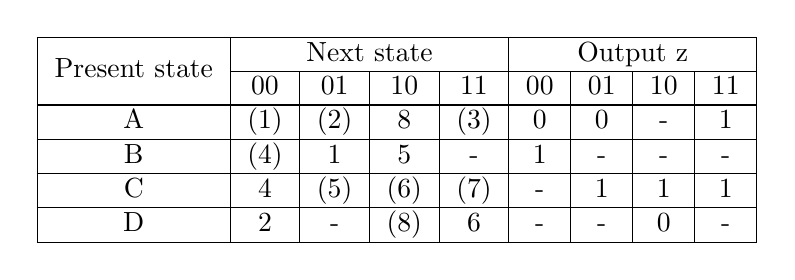
\begin{tikzpicture}
			\node(table)
			{
				\begin{tabular}{| c | c | c | c | c | c | c | c | c | c |}
					\hline
					\multirow{2}{*}{Present state} & \multicolumn{4}{c |}{Next state} & \multicolumn{4}{c |}{Output z} \\
					\cline{2-9} & $00$ & $01$ & $10$ & $11$ & $00$ & $01$ & $10$ & $11$ \\
					\hline
					A & (1) & (2) & 8 & (3) & 0 & 0 & - & 1 \\
					\hline
					B & (4) & 1 & 5 & - & 1 & - & - & - \\
					\hline
					C & 4 & (5) & (6) & (7) & - & 1 & 1 & 1 \\
					\hline
					D & 2 & - & (8) & 6 & - & - & 0 & -  \\
					\hline
				\end{tabular}
			};
		\end{tikzpicture}
	\end{center}
	
	Draw the transition diagram for current states:
	\begin{center}
		\begin{tikzpicture}
			\node(graphic)
			{
				\includegraphics{Q2bTD.pdf}
			};
		\end{tikzpicture}
	\end{center}
	
	No diagonal transition, assigning state directly:
	$$A=00$$
	$$B=01$$
	$$C=11$$
	$$D=10$$
	
	Excitation table:
	\begin{center}
		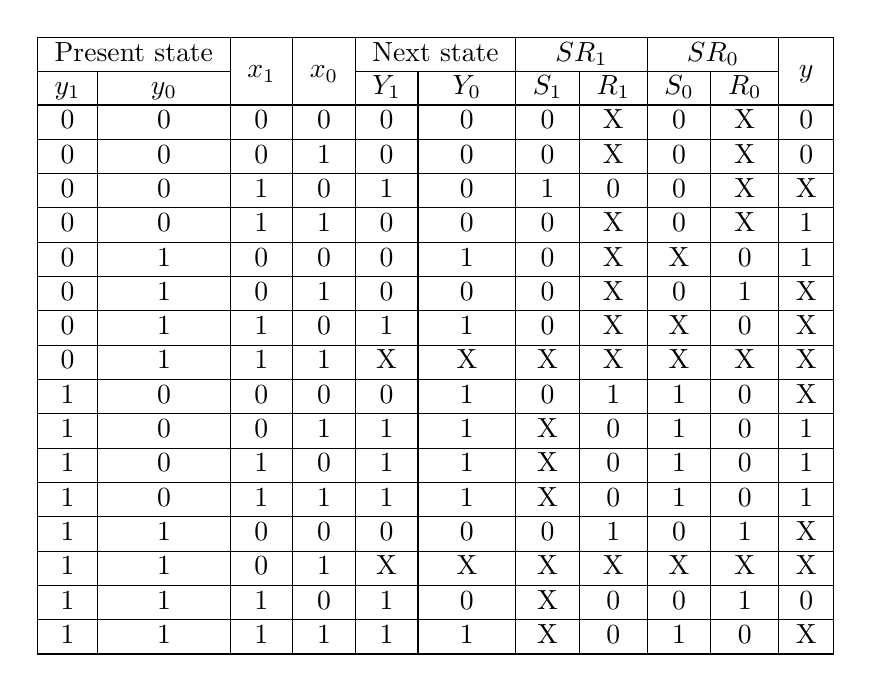
\begin{tikzpicture}
			\node(table)
			{
				\begin{tabular}{| c | c | c | c | c | c | c | c | c | c | c | c | c | c |}
					\hline
					\multicolumn{2}{| c |}{Present state} & \multirow{2}{*}{$x_1$} & \multirow{2}{*}{$x_0$} &\multicolumn{2}{c |}{Next state} & \multicolumn{2}{c |}{$SR_1$} & \multicolumn{2}{c |}{$SR_0$} & \multirow{2}{*}{$y$} \\
					\cline{1-2} \cline{5-10}
					$y_1$ & $y_0$ & & & $Y_1$ & $Y_0$ & $S_1$ & $R_1$ & $S_0$ & $R_0$ & \\
					\hline
					0 & 0 & 0 & 0 & 0 & 0 & 0 & X & 0 & X & 0 \\
					\hline
					0 & 0 & 0 & 1 & 0 & 0 & 0 & X & 0 & X & 0 \\
					\hline
					0 & 0 & 1 & 0 & 1 & 0 & 1 & 0 & 0 & X & X \\
					\hline
					0 & 0 & 1 & 1 & 0 & 0 & 0 & X & 0 & X & 1 \\
					\hline
					0 & 1 & 0 & 0 & 0 & 1 & 0 & X & X & 0 & 1 \\
					\hline
					0 & 1 & 0 & 1 & 0 & 0 & 0 & X & 0 & 1 & X \\
					\hline
					0 & 1 & 1 & 0 & 1 & 1 & 0 & X & X & 0 & X \\
					\hline
					0 & 1 & 1 & 1 & X & X & X & X & X & X & X \\
					\hline
					1 & 0 & 0 & 0 & 0 & 1 & 0 & 1 & 1 & 0 & X \\
					\hline
					1 & 0 & 0 & 1 & 1 & 1 & X & 0 & 1 & 0 & 1 \\
					\hline
					1 & 0 & 1 & 0 & 1 & 1 & X & 0 & 1 & 0 & 1 \\
					\hline
					1 & 0 & 1 & 1 & 1 & 1 & X & 0 & 1 & 0 & 1 \\
					\hline
					1 & 1 & 0 & 0 & 0 & 0 & 0 & 1 & 0 & 1 & X \\
					\hline
					1 & 1 & 0 & 1 & X & X & X & X & X & X & X \\
					\hline
					1 & 1 & 1 & 0 & 1 & 0 & X & 0 & 0 & 1 & 0 \\
					\hline
					1 & 1 & 1 & 1 & 1 & 1 & X & 0 & 1 & 0 & X \\
					\hline
				\end{tabular}
			};
		\end{tikzpicture}
	\end{center}
	
	Design equations:
	$$S_1 = x_1x_0' + y_1x_0$$
	$$R_1 = x_1'x_0'$$
	$$S_0 = y_1y_0' + y_1x_0$$
	$$R_0 = y_1'x_0 + y_1y_0x_0'$$
	$$y = y_1'x_1 + y_1'y_0 + y_1y_0'$$
	
	\section*{Question IV}
	\subsection*{Part a}
	Number two AND gates for disambiguation:
	\begin{center}
		\begin{tikzpicture}
			\node(graphic)
			{
				\includegraphics[scale=2]{Q4.png}
			};
		\end{tikzpicture}
	\end{center}
	
	Timing Diagram:
	\begin{center}
		\begin{tikzpicture}
			\node(graphic)
			{
				\includegraphics[scale=0.35]{Q4Timing.png}
			};
		\end{tikzpicture}
	\end{center}
	
	AND2 and OR will change output during the second gate delay period.
	\\
	
	At the beginning:
	
	the input of AND2 gate is (1, 1), so the output will change to 1;
	
	the input of OR gate is (0, 0), so the output will change to 0;
	\\
	
	During the second gate delay, the output of AND2 will gradually change from 0 to 1,
	and the output of OR will gradually change from 1 to 0. However, the output of AND2
	is one of the inputs of OR. The OR gate may thus generete an intermediate output 
	(labeled on the timing diagram), which may be neither 1 nor 0, creating a potential
	glitch in the system.
	
	\subsection*{Part b}
	Rewrite $f$ with minterms and maxterms:
	\begin{align*}
		f &= (w + z)(x' + z') + w'y \\
		&= wx' + wz' + zx' + w'y \\
		&= \sum{m(1,2,3,6,7,8,9,10,11,12,14)}
	\end{align*}
	\begin{align*}
		f &= (w + z)(x' + z') + w'y \\
		&= (x' + z' + w')(w + z + y)(x' + z' + y) \\
		&= \prod{M(0, 4, 5, 13, 15)}
	\end{align*}
	
	Recreate the K-map for $f$:
	\begin{center}
		\begin{tikzpicture}
			\node(table)
			{
				\includegraphics{Q4bK.pdf}
			};
		\end{tikzpicture}
	\end{center}
	
	Red circles are adjacent 1's who are not in the same group, indicating a static-1 hazard.
	Blue circles are adjacent 0's who are not in the same group, indicating a static-0 hazard.
	
	Redesigning for hazard-free:
	\begin{center}
		\begin{tikzpicture}
			\node(table)
			{
				\includegraphics{Q4bKhf.pdf}
			};
		\end{tikzpicture}
	\end{center}
	$$f = wx' + wz' + zx' + w'y + yz'$$
	
\end{document}
